\documentclass[format=acmsmall,screen,review,authordraft,nonacm]{acmart}
%\documentclass[format=acmsmall,screen,review,authordraft]{acmart}
%\documentclass{article}

% FIXME: https://arxiv.org/pdf/1709.06182.pdf
%        maja ladny template / chyba dziabne
%        albo ten z brytyjskiego sem6
%      https://github.com/borisveytsman/acmart

% FIXME: https://github.com/google-research/arxiv-latex-cleaner

% XXX: (mental anchor / looped / 3h) ->  UNDADASEA + LANE 8
%      https://www.youtube.com/watch?v=n_LcVqqHSY8
%      https://www.youtube.com/watch?v=vpeljtzB1a4

%\usepackage{arxiv}

\usepackage[utf8]{inputenc} % allow utf-8 input
\usepackage[T1]{fontenc}    % use 8-bit T1 fonts
%\usepackage[hidelinks]{hyperref}       % hyperlinks
\usepackage{url}            % simple URL typesetting
\usepackage{booktabs}       % professional-quality tables
\usepackage{amsfonts}       % blackboard math symbols
\usepackage{nicefrac}       % compact symbols for 1/2, etc.
\usepackage{microtype}      % microtypography
\usepackage{lipsum}		% Can be removed after putting your text content
\usepackage{graphicx}
\usepackage{float}

\usepackage{url}
\newcommand\longvar[1]{\mathchardef\UrlBreakPenalty=100
\mathchardef\UrlBigBreakPenalty=100\url{#1}}

%%% BONUS %%%
%\usepackage[table]{xcolor}  % for colors (like `red`)
\usepackage[normalem]{ulem} % for underline
\usepackage{booktabs}       % for better table
\usepackage{bm}             % for special table cell (`cellcolor`)
\usepackage{hhline,soul}    % for `hl` command (highlight text)
\usepackage{amsmath}        % for multi-line math
\usepackage[bottom]{footmisc}% for footnotes
\usepackage{tabularx, booktabs}
\newcolumntype{L}{>{\raggedright\footnotesize}m{6cm}}
\renewcommand{\arraystretch}{1.2}
%%%%%%%%%%%%%

%%% BIBTEX %%%
% https://sunsite.icm.edu.pl/pub/CTAN/info/biblatex-cheatsheet/biblatex-cheatsheet.pdf
%\usepackage[backend=bibtex, style=numeric, sorting=ynt]{biblatex}
%\addbibresource{main.bib} %                       `ynt` vs. `ydnt`
%\newcommand{\citep}[1]{\citeauthor*{#1} \cite{#1}} % for `fancy` cite style
%%%%%%%%%%%%%%

\newcommand{\ourjfasingle}{JFAStar}
\newcommand{\ourjfa}{Lord Vorotron} % okJFAuto / JFAstar
%\title{A survey of \emph{jump flooding algorithm} applied to Voronoi}
% \emph{\ourjfa}: Evolving Fast GPU Algorithm for
% Voronoi Diagram and Distance Transform in O(1) from JFA using AutoML
\title{lord vorotron: finding the best JFA variant for the coming winter} % $\approx$

%\renewcommand{\headeright}{}
%\renewcommand{\undertitle}{Draft}
%\renewcommand{\shorttitle}{\ourjfa}

%\date{September 9, 1985}	% Here you can change the date presented in the paper title
%\date{} 					% Or removing it


\author{Maciej A. Czyzewski}
\affiliation{%
 \institution{Poznan University of Technology}
 \city{Poznan}
 \country{Poland}}

\author{Kamil Piechowiak}
\affiliation{%
 \institution{Poznan University of Technology}
 \city{Poznan}
 \country{Poland}}


% \author{
%   Maciej A.~Czyzewski\\
%   Institute of Computing Science\\
%   Poznan University of Technology\\
%   Piotrowo 2, 60-965 Poznan, Poland\\
%   \texttt{maciejanthonyczyzewski@gmail.com} \\
%   \And
%   Kamil~Piechowiak\\
%   Institute of Computing Science\\
%   Poznan University of Technology\\
%   Piotrowo 2, 60-965 Poznan, Poland\\
%   \texttt{kamil.cams@gmail.com} \\
% }

\begin{document}

%%%%%%%%%%%%%%%%%%%%%%%%%%%%%%%%%%%%%%%%%%%%%%%%%%%%%%%%%%%%%%%%%%%%%%%%%%%%%%%%

\hl{\textbf{UWAGA!} Przenioslem fragmenty ze starego szkicu, teraz jednak czuje ze
powinnien byc to takie ogolne podsumowanie wszystkich mozliwych wariantow JFA - i
w jakich przypadkach sie sprawdzaja. A tak przyokazji nasza wersja z szumem+trikami
ktora dobrze dziala, no i dodatek taki ze mozna teraz zrobic sobie ensembla (a
nie jako glowny cel tej pracy). Dlatego wszystko co ponizej to praktycznie
random/bardzo mocny szkic. Wykresy to wizualizacja smaku.}
\newline

\begin{abstract}
This paper studies a practical usage of machine learning (AutoML) to automate
research towards discovering efficient Voronoi Diagram and Distance Transform
algorithms.  As the baseline we used the Jump Flooding Algorithm (JFA) - by
finding new mutations which works best for specific data, and then ensembling
them into one, we create new state-of-the-art algorithm in this field named
\textbf{\ourjfa} \hspace{0.01cm} with time complexity \textcolor{red}{$\approx$O(1)} and
work complexity \textcolor{red}{$\approx$O(N)}.
The algorithm is faster and produces more accurate approximations. It could be
extended into 3D space in a slice-by-slice manner.  We started from the
assumption that JFA has potential for improvement - some benefits can be
observed for specific data by adding random noise and adjusting the step size in
JFA.  This showed us that, AutoML could examine this space, and find the best
possible algorithm in each case.  In the further part of the work, we discuss
the results, compare the variants and ensemble for creating the final algorithm.
\end{abstract}

\maketitle

\hl{\textbf{CEL:} omawiamy dwa algorytmy? jeden nastepca JFA} -
\textbf{\ourjfasingle} \hspace{0.01cm} \hl{oraz ensembla po naszym score fn. -}
\textbf{\ourjfa}???????

\keywords{aaaaaaaaaaaaaaaaaa \and bbbbbbbbbbbbbbb \and ccccccccccccccccccc}

%%%%%%%%%%%%%%%%%%%%%%%%%%%%%%%%%%%%%%%%%%%%%%%%%%%%%%%%%%%%%%%%%%%%%%%%%%%%%%%%
\section{Introduction} %%%%%%%%%%%%%%%%%%%%%%%%%%%%%%%%%%%%%%%%%%%%%%%%%%%%%%%%%
%%%%%%%%%%%%%%%%%%%%%%%%%%%%%%%%%%%%%%%%%%%%%%%%%%%%%%%%%%%%%%%%%%%%%%%%%%%%%%%%

% FIXME: na wypadek zmiany tytulu w przyszlsoci!!!!!!!!!! ;-)
This paper\footnote{the original title for this paper was ``Lord Vorotron:
Finding the Best JFA Variant for the Coming Winter''} studies a practical usage of machine learning to automate research
towards discovering efficient Distance Transform algorithms (utilizing technique known as AutoML).
Thus, by finding mutations which works best for specific data, and then ensembling them into
one, we create new state-of-the-art algorithm in this field named \uline{\ourjfa \hspace{0.01cm} with
time complexity $\approx$O(1) and work complexity $\approx$O(N).}

Notable contribution to the quick algorithm that makes Distance Transform (DT)
using graphics hardware includes \citep{hoff1999fast} that creates a cone for
each input (point/seed) and renders those cones to obtain the Voronoi diagram as the lower envelope of these cones.
\cite{fischer2006fast} use planes tangent to a paraboloid and thus avoid the errors caused by the tessellation of the cones.
Unfortunately, the drawback of this approach is the significant amount of computation and the implementation complexity.

Jump flooding algorithm (JFA)\footnote{a novel pattern of
communication} is an interesting way to utilize the graphics processing unit to
efficiently compute Voronoi diagrams and distance transforms
\cite{rong2006jump}. This method is faster and produces more accurate results
\cite{rong2007variants}, and furthermore, it could be extended into 3D space in a slice-by-slice manner.
This is more effective than the previous research carried out by
\citep{sud2006interactive}, because the speed of JFA is almost independent to the number of seeds \cite{rong2007variants}.

Based on this research and findings, several efficient GPU-based algorithms which are either
work optimal or time optimal have been proposed including
SKW \cite{schneider2009gpu}, PBA \cite{cao2010parallel}, FastGPU \cite{de2017fast}, Honda's algorithm \cite{honda2017simple} and
WTO \cite{manduhu2019work}.

The main question that needs to be addressed now is whether JFA has potential
for improvement. We found some benefits for specific data by adding random noise
and adjusting the phase size in JFA. Therefore, this shows that, AutoML could examine this
unknown space, and find the best possible algorithm in each case.

For convenience, this work focus on the Voronoi diagram only - because this problem can be translated to DT \cite{rong2006jump}.
The algorithm would be an approximation of the output, thus we suggest using WTO
\cite{manduhu2019work} for exact DT (EDT). The major contributions of this paper are thus:

\begin{enumerate}
	\item Presenting new state-of-the-art variants of algorithm for Voronoi
		Diagram and Distance Transform: \newline
		\textbf{\ourjfasingle} - single best variant;
		\textbf{\ourjfa} - ensemble of weak variants; and
	\item Analyzing all possible variants of JFA: comparing error and speedup
		relative to bruteforce method
%\item Proposing, for an input set of seeds in a 2D grid, the first
%parallel algorithm in GPU to compute in constant time (i.e.
%independent of the number of seeds) a highly accurate
%Voronoi diagram and distance transform.
\end{enumerate}

%%%%%%%%%%%%%%%%%%%%%%%%%%%%%%%%%%%%%%%%%%%%%%%%%%%%%%%%%%%%%%%%%%%%%%%%%%%%%%%%
\section{Related Work} %%%%%%%%%%%%%%%%%%%%%%%%%%%%%%%%%%%%%%%%%%%%%%%%%%%%%%%%%
%%%%%%%%%%%%%%%%%%%%%%%%%%%%%%%%%%%%%%%%%%%%%%%%%%%%%%%%%%%%%%%%%%%%%%%%%%%%%%%%

Several efficient GPU-based algorithms which are either
work optimal or time optimal have been proposed including
JFA \cite{rong2006jump}, SKW \cite{schneider2009gpu},
PBA \cite{cao2010parallel}, FastGPU \cite{de2017fast}, Honda's algorithm \cite{honda2017simple} and
WTO \cite{manduhu2019work}.

\begin{table}[H] \centering
\begin{tabular}{@{}lllll@{}}
\toprule
Reference                & Algorithm    & Exactness   & Time         & Work         \\ \midrule
\citep{de2017fast}       & FastGPU      & Exact       & $O(n^3/p)$   & -            \\
\citep{cao2010parallel}  & PBA          & Exact       & $O(n)$       & $O(mN)$      \\
\citep{honda2017simple}  & based on SKW & Exact       & $O(n)$       & $O(N)$       \\
\citep{manduhu2019work}  & WTO          & \cellcolor{blue!25}\textbf{Exact}& \cellcolor{blue!25}$\bm{O(\log n)}$  & $O(N)$       \\
\citep{schneider2009gpu} & SKW          & Approximate & $O(n)$       & $O(N)$       \\
\citep{rong2006jump}     & JFA          & Approximate & $O(\log n)$  & $O(N\log n)$ \\ \bottomrule
In this paper            & \ourjfa      & \cellcolor{blue!25}\textbf{Approximate} & \cellcolor{blue!25}$\sim$$\bm{O(1)}$ & $\sim$$O(N)$ \\ \bottomrule
\end{tabular}
\vspace{1em}
\caption{Different GPU algorithms for computing EDT}
\end{table}

\subsection{Jump Flooding} %%%%%%%%%%%%%%%%%%%%%%%%%%%%%%%%%%%%%%%%%%%%%%%%%%%%%

\hl{redukcja i bridge pomiedzy intro (usunac subsection)}

co to jest jump flooding? tak naprawde to nie jest algorytm do voronoi-a tylko
pattern komunikacyjny w programowaniu rownoleglym - swojej pracy doktorskiej
autor tej techniki podaje wiele zastosowan jednak w swoich badaniach ogranicza
sie do Voronoi-a. glownym pytaniem roznych takich patternow jest ile potrzebnych
jest rund/operacji komunikacji aby zagwarantowac aby dana informacja zostanie
dostarczona. akurat w voronoi-u wiele komorek jest lokalna w skali calego
przykladu - wiec JFA ktora gwarantuje dostarczenie informacji globalnie do
kazdego punktu - wykonuje pewne niepotrzebne operacje.  szybkosc i zajetosc
pamieciowa JFA jest satysfakcujaca, jednak proste modyfikacje pokazuja ze
algorytm ten wykonuje sie szybciej w pewnych przypadkach (i to typowych).
dlatego naturalnym pytanie powinno byc w jakich oraz jakie modyfikacje wplywaja
na szybkosc dzialania.

\subsection{AutoML} %%%%%%%%%%%%%%%%%%%%%%%%%%%%%%%%%%%%%%%%%%%%%%%%%%%%%%%

\hl{przeniesc do Proposed Method}

\url{https://arxiv.org/pdf/1801.09373.pdf}
\url{https://arxiv.org/pdf/1804.10120.pdf}
\url{https://arxiv.org/pdf/1703.06353.pdf}

okay przenioslem - dodac prace co tez tak szuka algosow

%%%%%%%%%%%%%%%%%%%%%%%%%%%%%%%%%%%%%%%%%%%%%%%%%%%%%%%%%%%%%%%%%%%%%%%%%%%%%%%%
\section{Proposed Method} %%%%%%%%%%%%%%%%%%%%%%%%%%%%%%%%%%%%%%%%%%%%%%%%%%%%%%
%%%%%%%%%%%%%%%%%%%%%%%%%%%%%%%%%%%%%%%%%%%%%%%%%%%%%%%%%%%%%%%%%%%%%%%%%%%%%%%%

\hl{przepisac ten szkic bo jezyk sie placzy}

JFA opiera sie na tym ze infomacja jest przekazywana ??????.  Przekazanie odbywa
sie w log(n) krokach. Wiec przeprowadzilismy krotki eksperyment applyujac losowy
szum na wejsciowa masce. Okazalosie sie ze ilosc potrzebnych krokow spadla -
powstaly losowe shortcuty.  Co oznacza ze powinny istniec inne "mutacje"
algorytmow lepsze w pewnych okreslonych przypadkach.  Wiec szukanie najszybszego
algorytmu bedzie nastepujace:

\begin{itemize}
\item Wymyslenie wszystkich mozliwych wariantow JFA
\item Mutacje i zapisanie najlepszych wersji dla danej domeny
\item Ensemblacja algorytmow tak aby wybierac najlepszy variant dla danej domeny
\end{itemize}

\subsection{Domain Space} %%%%%%%%%%%%%%%%%%%%%%%%%%%%%%%%%%%%%%%%%%%%%%%%%%%%%%

\hl{okay, zupelnie inaczej tutaj podejsc, opisac jakie sa przypadki i jakie sa
spotykane}

jakie domeny i dlaczego (i jak dzialaly gen\_uniform, \hl{gen\_polar, gen\_grid})

\subsection{Search Space} %%%%%%%%%%%%%%%%%%%%%%%%%%%%%%%%%%%%%%%%%%%%%%%%%%%%%%

\hl{bridge z score function gdziekolwiek to bedzie}
\hl{obliczyc ile jest aktulanie wersji algosow np. czy jest to juz 2do14 jak
mamy 3xreal w wielomianie AKTUALNIE JEST okolo 7,200?}

jakie modyfikacje, na to osobna sekcja? wiec co tu napisac
chyba tylko o zlozonosci problemu i ze kod jest skladany i testowany a niektore
wersje sa pomijane zgodnie z dzialaniem gp\_minimize (Bayesian optimization
using Gaussian Processes).

w naszym wypadku zdefiniowalismy pewien zbior variantow pewnych czesci
algorytmu (Search Space), modul testujacy dana mutacje/wariant - sklada kod kernela a pozniej go weryfikuje na naszej Domain Space.

\subsection{Score Function} %%%%%%%%%%%%%%%%%%%%%%%%%%%%%%%%%%%%%%%%%%%%%%%%%%%

\hl{SCORE CZY METRIC?}
\hl{roznica w pikselach pomiedzy bruteforce a algorytmem - napisac o tym / tez
ze to wszystko to ilorazy do bruteforce}

dla voronoi-a interesuja nas 2 parametry Error oraz Szybkosc, aby wyniki byly
wiarygodne porownujemy je z bruteforcem (a wiec bedzie to iloraz).
aby ocenic dana mutacje musimy przypisac jakis Score danej wersji, wiec uzylismy
wzor ponizej

\begin{align}
	S(x,y) = max\{0, \sqrt{x} \cdot (100-y^{2})\}, \\
0 \leq y \leq 100, 0 < x
\end{align}

ktory kaze za zbyt wysokie errory, dajac zerowy wynik - skladnik przy y rosnie
szybciej niz x wiec gdy przekroczy 100 da nam ujemny wynik - czyli 0.

\subsection{Optimizer} %%%%%%%%%%%%%%%%%%%%%%%%%%%%%%%%%%%%%%%%%%%%%%%%%%%%%%%%%

\hl{opisac dwie osobne taktyki optymalizacji dla best single vs. ensemble}

mozemy napisac ze korzystalismy z forest/gp minimize, ale tez wspomniec ze aby
miec najlepszy best single to trzeba bylo optymalizowac rownoczesnie cala
przestrzen (od malych do duzych, gestych po rzadkie), a zeby miec najlepszego
Vorotrona - czyli ensembla to trzeba bylo dla kazdej domeny z optymalizowac a
pozniej jedynie zrobic balancera!!!!!!!!!!!!

\hl{trzeba to przeszukiwac tak aby nie sfiksowal na zadanych parametrach - bo
niechcacy ocenia na poczatku ze szum/dual jest nie fajny i pozniej go juz nie
rozwaza}

\subsection{Ensemble} %%%%%%%%%%%%%%%%%%%%%%%%%%%%%%%%%%%%%%%%%%%%%%%%%%%%%%%%%%

\hl{mozna zapisac tabele dla kazdej domeny (shape) / i zrobic przewidywania
parametrow (slownik wariantu) - bo dla malych oplacalne sa Circle6 a dla
wiekszych Circle12 i tak dalej - jak to zrobic?}

patrzac na rezultaty mozemy znalesc jaki algorytm najlepiej sprawdza sie w
zadanej domenie. np. widac ze dla malej ilosci seedow (malo gestych przypadkow,
ktore maja mala powierzchnie) oplaca sie uzyc bruteforce. Dla kolejnych
wiekszych przypadkow innych wariantow JFA. Jak wybrac algorytm? Kazdy przypadek ma `shape` oraz `num` wiec mozna na CPU wysemplowac
pare punktow albo odrazu obliczyc gestosc i wybrac odpowiedni algorytm.
To takich ensemblacji najlepiej sprawdzi sie drzewo decyzyjne (moze byc boostowane).

%%%%%%%%%%%%%%%%%%%%%%%%%%%%%%%%%%%%%%%%%%%%%%%%%%%%%%%%%%%%%%%%%%%%%%%%%%%%%%%%
\section{Variants} %%%%%%%%%%%%%%%%%%%%%%%%%%%%%%%%%%%%%%%%%%%%%%%%%%%%%%%%%%%%%
%%%%%%%%%%%%%%%%%%%%%%%%%%%%%%%%%%%%%%%%%%%%%%%%%%%%%%%%%%%%%%%%%%%%%%%%%%%%%%%%

\hl{ZROBIC LADNE RYSUNECZKI w Google Slides - eksport to pdf!}

To compute the Voronoi diagram for a 2D grid of size n×n
with a given set of seeds at some grid points, we are interested to
propagate the content (in particular, position information) of each
seed s to each grid point so that each grid point can decide which
seed is its closest one.

Niektore operacje propagacji informacji sa zbedne - tylko w przypadkach
rzadkich macierzy potrzeba jest log(n) krokow aby uzyskac prawidlowy wynik.
Rozne warianty omawiane w \cite{rong2007variants} pozwalaja zredukowac blad
klasycznego JFA. Nie zostaly jednak omawiane przypadki gdzie poszczegolne
modyfikacje sa uzywane z innymi.

Dlatego w tej pracy prezentujemy dodatkowe modyfikacje ktore mozna zastosowac
aby stworzyc nowe warianty. Pewne modyfikacje sa oczywiste i wynikaja z
alternatywnego podejscia (zamiast anchoru\footnote{anchorem nazywamy metode
ktora pobiera sasiadow do przekazania informacji} kwadratowego mozna uzyc kola),
informacje mozna wstepnie rozpropagowac losowo - w nadzie ze pozwoli nam
skonczyc algorytm w mniejszej ilosci krokow.

Aby badania byly bardziej przejrzyste trzymalismy sie pewnej konfencji
nazewniczej:

$$
[\bm{anchor\_type}][\bm{anchor\_num}][\bm{anchor\_double}]\qquad|\qquad[\bm{step\_function}]\qquad+\qquad[\bm{noise}]
$$

dla przykladu \textit{Circle11(1/3)Dual(1/4)|Factor3+Noise} ktore mozna
przeczytac jako:

\begin{multline}
anchor\_type=Circle, anchor\_num=11, anchor\_number\_ratio=1/3, \\
anchor\_double=True, anchor\_distance\_ratio=1/4, \\
step\_function=Factor3, noise=True
\end{multline}

\subsection{Noise} %%%%%%%%%%%%%%%%%%%%%%%%%%%%%%%%%%%%%%%%%%%%%%%%%%%%%%%%%%%%%

\hl{FIXME: figure z przykladami szumu (+local) i jak to wyglada i jak wygladalo
instancja!}

Zamiast zaczynac od pustej macierzy z seed-ami poczatkowymi mozna ja losowa
uzupelnic szumem - tworzac przypadkowe short-cuty. Mozna tego dokonac osobnym
kernelem ktory zostatnie wywolany przed wykonaniem glownej czesci algorytmu.
Interpretacja jest taka ze pewne rejony ktora w JFA sa wypelnione zerami podczas
pierwszych iteracji nie podejmuja zadnych decyzji. Uzupelniajac szumem moga one
przypadkowo ustawic sie na prawidlowa wartosc i propagowac w kolejnej rundzie
najlepsza wartosc w swoim otoczeniu (zgodnie ze stepem).

\hl{dowod kamila tutaj????????????????}

\subsubsection{Local Noise} %%%%%%%%%%%%%%%%%%%%%%%%%%%%%%%%%%%%%%%%%%%%%%%%%%%%%%%

Mozna tez szum uzupelniac nie losowo tylko w otoczeniu. Wiec gdy w punkcie
$(x,y)$ wylosujemy losowego seed-a o wartosci $(x_{rand}, y_{rand})$ to
wyliczamy nowa pozycje $(x', y')$ ktora znajduje sie
w polowie drogi w nastepujacy sposob: $x' = \frac{x+x_{rand}}{2}$, analogicznie
dla $y'$. Dodatkowo jesli $(x', y')$ jest pusta to tez uzupelniamy to pole ta
informacja. Nie przejmujemy sie wyscigiem w dostepie do danych. Nadpisania beda
losowe - a szum tez.

\subsection{Anchor Type} %%%%%%%%%%%%%%%%%%%%%%%%%%%%%%%%%%%%%%%%%%%%%%%%%%%%%%%

\hl{losowane punkty na okregu???}

Zamiast pobierac informacje od 8 sasiadow o step size from grid points at
$(x+i, y+j)$ where $i, j \in \{-\text{step}, 0, \text{step}\}$. Mozna zastosowac
okrag - otwiera nam to nowe mozliwosci na swobodna modyfikacje ilosci punktow od
ktorych bedziemy pobierac informacje. Naturalnie wydaje sie ze mala ilosc
punktow w anchorze spowoduje wzrost bledu, a duza ilosc punktow spowoduje
zmalenie bledu.

\subsubsection{Anchor Num} %%%%%%%%%%%%%%%%%%%%%%%%%%%%%%%%%%%%%%%%%%%%%%%%%%%%%%%%

Dlatego kolejnym parametrem bedzie mozliwosc kontrolowania ilosci punktow.
Niestety nie rozwazalismy wariantu kwadratow o dowolnej ilosci punktow (poniewaz
byly by to wielokrotnosci 2x2=4, 3x3=9, 4x4=16, 5x5=25) bo i tak nie dalo by sie
wybrac uniformly tej wartosci. Dla okregu punkty sasiada $(x_i, y_i)$ byly liczone
nastepujaco:
   
$$
x_i = x + \text{step} \cdot \cos( \frac{2\pi}{\text{[anchor\_num]}} \cdot i ),
y_i = y + \text{step} \cdot \sin( \frac{2\pi}{\text{[anchor\_num]}} \cdot i )
$$

\subsection{Anchor Double} %%%%%%%%%%%%%%%%%%%%%%%%%%%%%%%%%%%%%%%%%%%%%%%%%%%%%

Oprocz pojedynczego anchora, mozliwe jest uzycie podwojnej warstwy anchorow
(czyli np. male kolko i wieksze). Idea za tym stojaca to ze male kolko
wewnetrzne jest dokladne (dziala jak w JFA) - a wielkie zewnetrzne
jest skautujace lub aby poprawic error wynikajacy np. z mniejszej ilosci
$\text{anchor\_num}$ (w sumie to podobny mechanizm jak w Lookahead - wolny/szybki)

\subsubsection{Anchor Distance Ratio}

Parametr mowiacy o stosunku dlugosci step size od wewnetrzengo anchora do
zewnetrznego.

\subsubsection{Anchor Number Ratio}

Parametr mowiacy o statusnku ilosci detektorow od wewnetrznego anchora do
zewnetrznego.

\subsection{Step Function} %%%%%%%%%%%%%%%%%%%%%%%%%%%%%%%%%%%%%%%%%%%%%%%%%%%%%

Gdy nasza informacja propaguje sie szybciej lub jest bardziej zageszczona
dlatego sasiedzi szybciej dostaja prawidlowa informacje - to oznacza ze mozna
skrocic ilosc round wykonania algorytmu.

Step size jak i ich ilosc mozna okreslic za pomoca 2 podstawowych parametrow:
shape and number of points - z ktorych pozniej mozemy okreslic np. srednia
gestosc. Zaimplementowalismy 2 warianty ktore sa uzaleznione jedynie od shape:
defaultowy z JFA, z JFA o podstawie 3; oraz jeden uzaleniony od shape oraz od num: logstar.
Jednak aby wygeneralizowac problem stworzylismy tez mozliwosc wygenerowania
dowolnego polynomialu.

\subsubsection{Special Polynomial}

\hl{problem z Special - on overfituje przyklady zmieniajac 5 miejsce po
przecinsku aby 2 zamienialo sie np. w 1}

Implementacja nie jest wazna - chodzi o idea zwiazania shape oraz num. Oraz
modyfikowanie wartosci, szybkosci spadku, ksztaltu (np. piloksztnego) - jakimis
parametrami. Wada tego rozwiazania jest ze trzeba optymalizowac ta funkcje na
calej dziedzinie (malej, duzej, gestej, zadkiej) - bo inaczej z overfituje ona
ilosc krokow i wiekosc stepu pod rozmiar.

%%%%%%%%%%%%%%%%%%%%%%%%%%%%%%%%%%%%%%%%%%%%%%%%%%%%%%%%%%%%%%%%%%%%%%%%%%%%%%%%
\section{Results} %%%%%%%%%%%%%%%%%%%%%%%%%%%%%%%%%%%%%%%%%%%%%%%%%%%%%%%%%%%%%%
%%%%%%%%%%%%%%%%%%%%%%%%%%%%%%%%%%%%%%%%%%%%%%%%%%%%%%%%%%%%%%%%%%%%%%%%%%%%%%%%

\hl {przeniesc legende? JAKO OSOBNY PDF? i podac w tej sekcji - tak sie nie robi
ale bylo by ok i czytelnie + wiecej miejsca na wykresy a przypadkow bedzie
wiecej}
\hl{czy wykres loss oraz score dla przypadkow powinnien byc nalozony? albo
polaczony subfigurem tak aby osie byly sync. i dalo sie porownac}

performance plot\footnote{wykres zostal zrobiony poprzez posortowanie scorow - dzieki temu widac roznice w
przyroscie i latwo dostrzec ktory algorytm ma najwyzszy score lub jaka ma
chaktersytyke (np. jest bardzo skuteczny dla waskiej grupy przykladow)
}

\subsection{Multi-domain Algorithm (JFAStar)} %%%%%%%%%%%%%%%%%%%%%%%%%%%%%%%%%%

\begin{itemize}
	\item \textbf{shapes}: \{32x32, 64x64, 96x96, 128x128, 256x256, 320x320, 384x384, 448x448, 512x512, 768x768, 1024x1024, 1536x1536\}
	\item \textbf{cases}:
        \begin{itemize}
			\item gen\_uniform: seeds=1,
			\item gen\_uniform: seeds=2,
			\item gen\_uniform: density=0.0001,
			\item gen\_uniform: density=0.001,
			\item gen\_uniform: density=0.01,
			\item gen\_uniform: density=0.02,
			\item gen\_uniform: density=0.03,
			\item gen\_uniform: density=0.04,
			\item gen\_uniform: density=0.05,
			\item gen\_uniform: density=0.1,
		\end{itemize}
\end{itemize}

\begin{figure}[H]
	\centering
	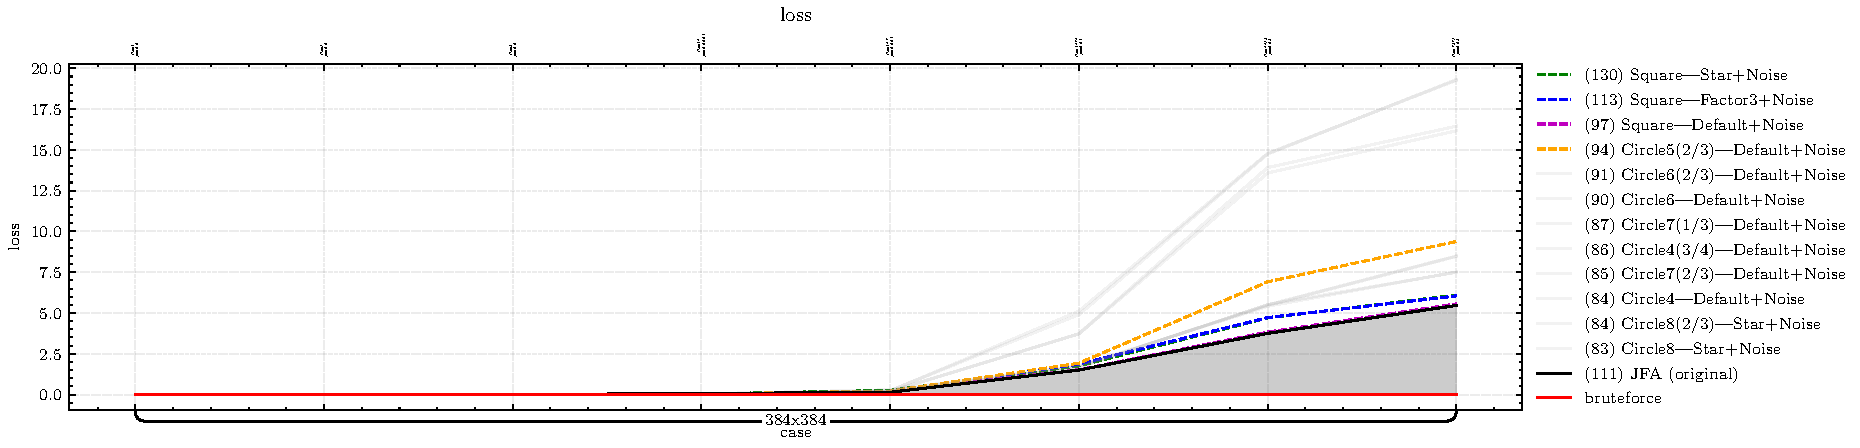
\includegraphics[width=\linewidth]{../figures/figure-2-loss}
	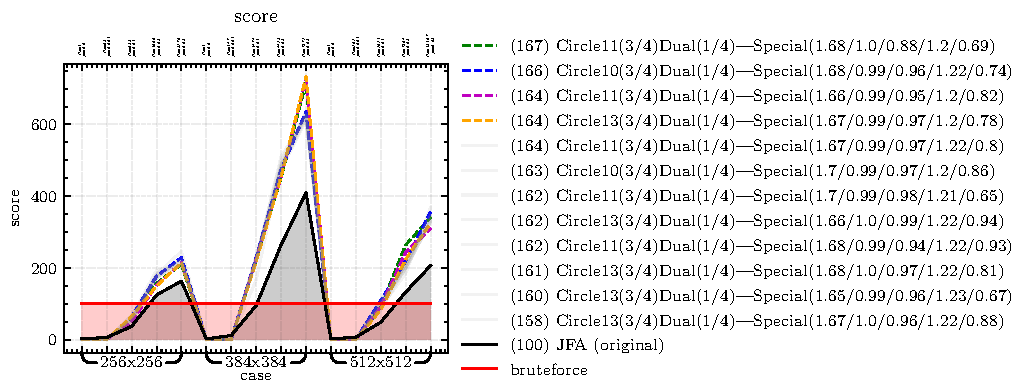
\includegraphics[width=\linewidth]{../figures/figure-3-score}
	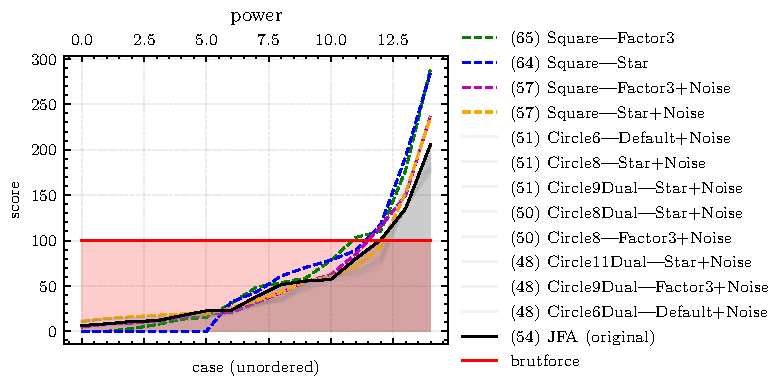
\includegraphics[width=\linewidth]{../figures/figure-4-power}
	\caption{bla bla bla}
	\label{fig:abstract}
\end{figure}

\begin{table}[H]
	\centering
	%\hspace*{-1cm}
	\begin{tabular}{lrrrllr}
\hline
 Algorithm                  &   $\rho$=0.0003 &   $\rho$=0.001 &   $\rho$=0.0099 & $\rho$=0.0298   & $\rho$=0.0499   &   Avg. score \\
\hline
 Square|Factor3             &             0   &           13.2 &            55.5 & \textbf{122.0}  & \textbf{169.3}  &           71 \\
 Square|Star                &             0   &            0   &            41.7 & \textbf{115.2}  & \textbf{161.5}  &           63 \\
 Square|Star+Noise          &            12.3 &           19   &            48.4 & 96.3            & \textbf{142.3}  &           63 \\
 Square|Factor3+Noise       &             7.9 &           13.6 &            43.5 & 91.6            & \textbf{145.2}  &           60 \\
 Circle8Dual|Default        &             0   &            9.8 &            39.3 & 85.6            & \textbf{123.3}  &           51 \\
 Circle10|Star+Noise        &            11.8 &           16.3 &            43.4 & 79.2            & 98.7            &           49 \\
 Circle10Dual|Factor3+Noise &             5.5 &           10.9 &            37.8 & 81.4            & \textbf{110.6}  &           49 \\
 Circle8Dual|Factor3+Noise  &             6.8 &           12.7 &            42.2 & 82.7            & 94.2            &           47 \\
 Circle10Dual|Star          &             0   &            0   &            28.2 & 85.0            & \textbf{124.2}  &           47 \\
 Circle11Dual|Factor3+Noise &             6   &           12   &            35.2 & 76.9            & \textbf{107.2}  &           47 \\
 Circle10Dual|Factor3       &             0   &            4.8 &            40.8 & 80.2            & \textbf{109.3}  &           47 \\
 Circle12|Star+Noise        &            10.6 &           14.7 &            37   & 70.3            & 87.2            &           43 \\
 Circle13|Factor3+Noise     &             6.2 &           10.4 &            32.6 & 70.9            & 92.2            &           42 \\
 Circle15Dual|Star          &             0   &            1.6 &            35.8 & 68.2            & \textbf{101.9}  &           41 \\
 Circle17Dual|Star          &             0   &            1.3 &            34.4 & 65.0            & 95.4            &           39 \\
 Circle6|Factor3+Noise      &             7.7 &           15.7 &            53.2 & 79.6            & 34.9            &           38 \\
 Circle7Dual|Default        &             0   &            6.4 &            37   & 66.7            & 79.7            &           37 \\
 Circle6Dual|Default        &             0   &            4.8 &            36.2 & 67.2            & 79.0            &           37 \\
 Circle6Dual|Star+Noise     &            14.7 &           20.9 &            42.1 & 59.2            & 32.4            &           33 \\
 Circle8Dual|Star           &             0   &            0   &             0   & 49.0            & 78.7            &           25 \\
 Circle9Dual|Star           &             0   &            0   &             0.2 & 39.1            & 74.9            &           22 \\
 Circle9Dual|Factor3        &             0   &            0   &             5.4 & 35.9            & 69.9            &           22 \\
 SquareDual|Factor3         &             0   &            4.9 &            19.2 & 35.8            & 49.8            &           21 \\
 Circle8Dual|Factor3        &             0   &            0   &             5.8 & 37.6            & 64.2            &           21 \\
 Circle10|Factor3           &             0   &            1.1 &            12.9 & 32.5            & 52.6            &           19 \\
 Circle14|Factor3           &             0   &            1   &            10.7 & 36.4            & 50.1            &           19 \\
 Circle9|Factor3            &             0   &            1.1 &             9.5 & 31.6            & 46.0            &           17 \\
 Circle10|Star              &             0   &            0   &             2.8 & 30.9            & 49.0            &           16 \\
 SquareDual|Default+Noise   &             2.1 &            3.5 &            12.3 & 26.7            & 37.8            &           16 \\
 Circle7Dual|Factor3        &             0   &            0   &             0   & 2.5             & 0.0             &            0 \\
 Circle7Dual|Star           &             0   &            0   &             0   & 1.9             & 0.0             &            0 \\
 Circle6Dual|Star           &             0   &            0   &             0   & 0.0             & 0.1             &            0 \\
\hline
\end{tabular}
	\newline
	\caption{domain: 32x32, 64x64, 128x128, 256x256}
\end{table}

\subsection{Specific-domain Algorithm} %%%%%%%%%%%%%%%%%%%%%%%%%%%%%%%%%%%%%%%%%

\subsubsection{32x32, 64x64, 96x96, 128x128}

\subsubsection{256x256, 320x320, 384x384, 448x448}

\subsubsection{512x512, 768x768, 1024x1024, 1536x1536}

\subsubsection{Low Density}

\subsubsection{High Density}

\subsection{Ensemble Across Domains (Vorotron)} %%%%%%%%%%%%%%%%%%%%%%%%%%%%%%%%

bla bla

\subsection{Objectives} %%%%%%%%%%%%%%%%%%%%%%%%%%%%%%%%%%%%%%%%%%%%%%%%%%%%%%%%

\hl{naprawic generowanie tego wykresu}
\hl{napisac co nie moze byc uzyte z czym?}

czyli co ma wplyw na co (w sumie to najwazniejsze mialo byc w pracy)

\begin{figure}[H]
	\centering
	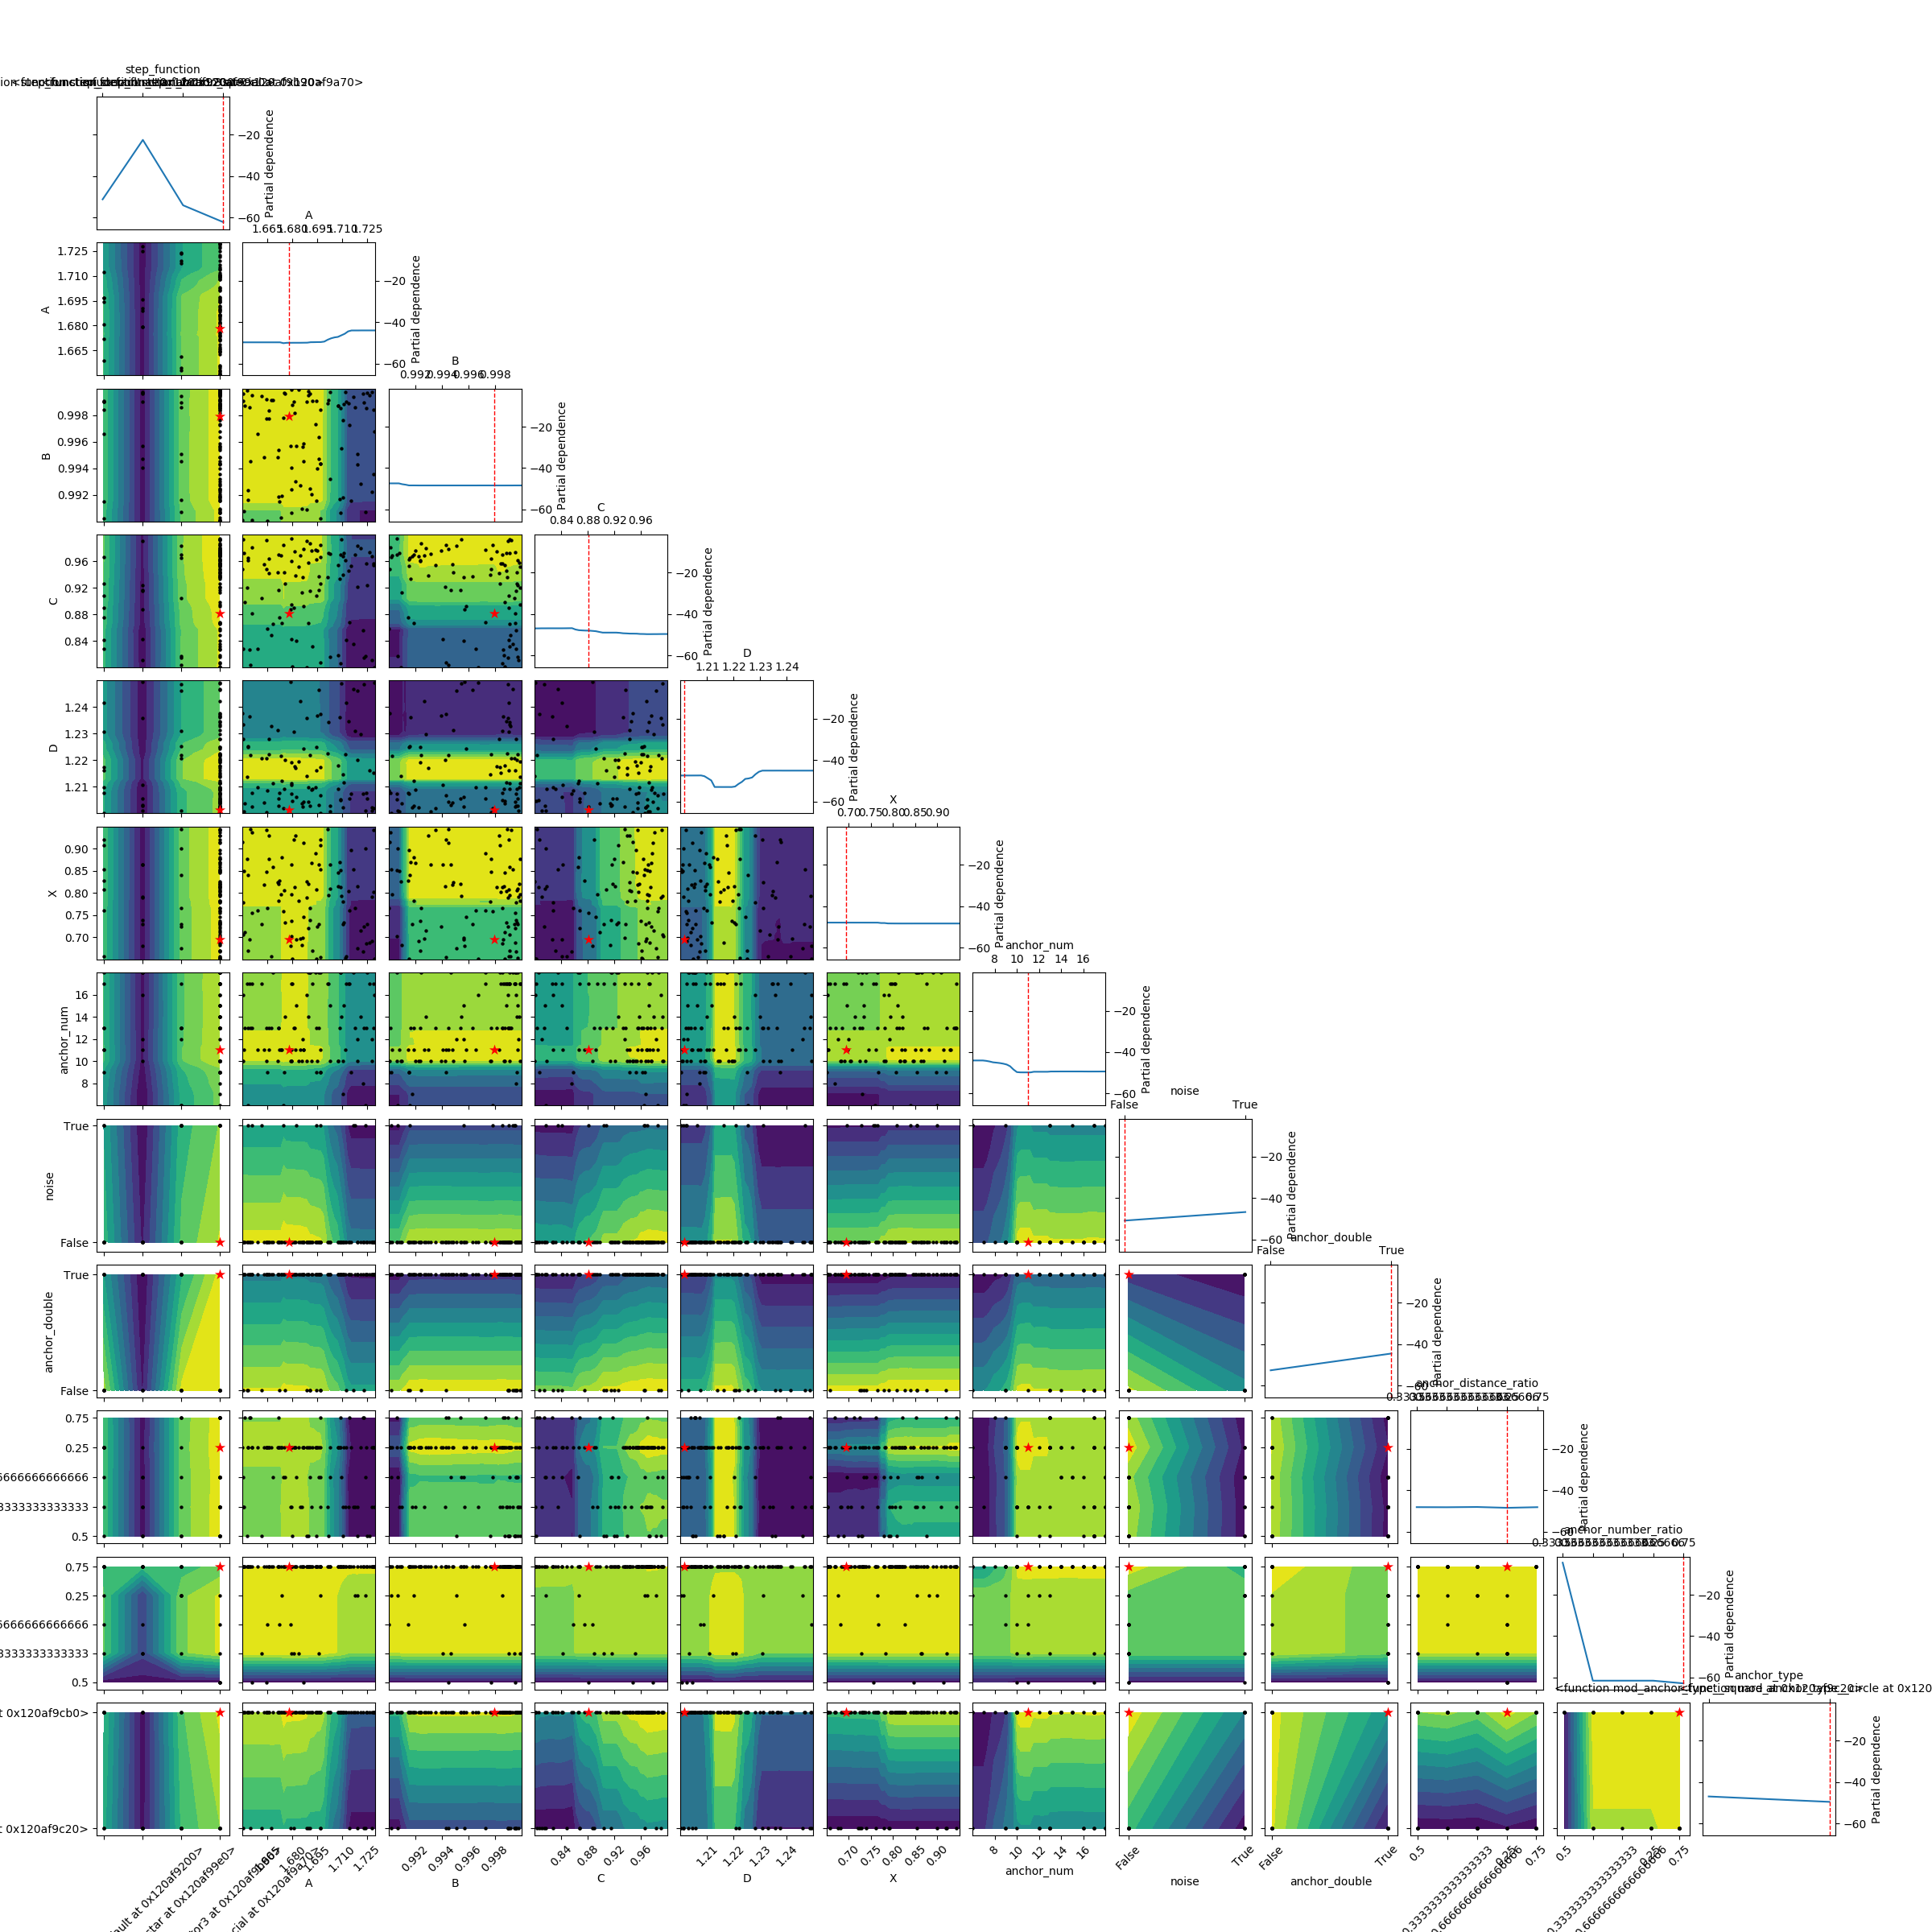
\includegraphics[width=\linewidth]{../figures/raport}
	\caption{bla bla bla}
	\label{fig:abstract}
\end{figure}

%%%%%%%%%%%%%%%%%%%%%%%%%%%%%%%%%%%%%%%%%%%%%%%%%%%%%%%%%%%%%%%%%%%%%%%%%%%%%%%%
\section{Practical Usage} %%%%%%%%%%%%%%%%%%%%%%%%%%%%%%%%%%%%%%%%%%%%%%%%%%%%%%
%%%%%%%%%%%%%%%%%%%%%%%%%%%%%%%%%%%%%%%%%%%%%%%%%%%%%%%%%%%%%%%%%%%%%%%%%%%%%%%%

\hl{polaczyc z Conclusions}

Jest wiele projektow ktore potrzebuje DT lub voronoi-a. Jedyne dwa praktyczne
przyklady z tej pracy to SOTA dla JFA - czyli JFAstar, oraz praktyczny Ensemble
(uwzgledniajacy np. bruteforce dla malych instancji).

%%%%%%%%%%%%%%%%%%%%%%%%%%%%%%%%%%%%%%%%%%%%%%%%%%%%%%%%%%%%%%%%%%%%%%%%%%%%%%%%
\section{Conclusions} %%%%%%%%%%%%%%%%%%%%%%%%%%%%%%%%%%%%%%%%%%%%%%%%%%%%%%%%%%
%%%%%%%%%%%%%%%%%%%%%%%%%%%%%%%%%%%%%%%%%%%%%%%%%%%%%%%%%%%%%%%%%%%%%%%%%%%%%%%%

This paper presents the GPU's effective, almost constant, algorithm for calculating the Euclidean distance transform (DT) approximation for 2D and higher dimensional images.
%
As mentioned in \cite{cao2010parallel}, it remains challenging to balance the workload in such an approach.
%
\textit{\ourjfa} does not explicitly solve this issue but, by constructing an alternative solution utilizing random shortcuts and parameter estimation, it makes it a reasonable approximation.
%
In practice, such a constant time algorithm is useful in many interactive applications, such as tessellations, rendering, and image processing, involving \cite{rong2006jump}.

%%%%%%%%%%%%%%%%%%%%%%%%%%%%%%%%%%%%%%%%%%%%%%%%%%%%%%%%%%%%%%%%%%%%%%%%%%%%%%%%
\section{Acknowledgements} %%%%%%%%%%%%%%%%%%%%%%%%%%%%%%%%%%%%%%%%%%%%%%%%%%%%%
%%%%%%%%%%%%%%%%%%%%%%%%%%%%%%%%%%%%%%%%%%%%%%%%%%%%%%%%%%%%%%%%%%%%%%%%%%%%%%%%

\hl{Dziekuje swojemu psu!Dziekuje swojemu psu! Dziekuje swojemu psu! Dziekuje swojemu psu! Dziekuje swojemu psu! Dziekuje swojemu psu! Dziekuje swojemu psu! Dziekuje swojemu psu! Dziekuje swojemu psu! Dziekuje swojemu psu! Dziekuje swojemu psu! Dziekuje swojemu psu! Dziekuje swojemu psu! Dziekuje swojemu psu! Dziekuje swojemu psu! Dziekuje swojemu psu! Dziekuje swojemu psu! Dziekuje swojemu psu! Dziekuje swojemu psu! Dziekuje swojemu psu! Dziekuje swojemu psu! Dziekuje swojemu psu! Dziekuje swojemu psu! Dziekuje swojemu psu!  }

%%%%%%%%%%%%%%%%%%%%%%%%%%%%%%%%%%%%%%%%%%%%%%%%%%%%%%%%%%%%%%%%%%%%%%%%%%%%%%%%

%\printbibliography
\bibliographystyle{ACM-Reference-Format}
\bibliography{main}

\end{document}
